\documentclass[conference]{IEEEtran}
\IEEEoverridecommandlockouts
% The preceding line is only needed to identify funding in the first footnote. If that is unneeded, please comment it out.
\usepackage{cite}
\usepackage{amsmath,amssymb,amsfonts}
\usepackage{algorithmic}
\usepackage{graphicx}
\usepackage{textcomp}
\usepackage{xcolor}
\usepackage{hyperref}
\def\BibTeX{{\rm B\kern-.05em{\sc i\kern-.025em b}\kern-.08em
    T\kern-.1667em\lower.7ex\hbox{E}\kern-.125emX}}
\begin{document}

\title{Analyzing the Effects of Weather}
\author{
\IEEEauthorblockN{Erens, Sam}
\IEEEauthorblockA{
  \textit{Department of Mathematics} \\
  \textit{Department of Statistics} \\
  \textit{University of Illinois, Champaign} \\
  Champaign, IL, United States \\
  serens2@illinois.edu
}
\and
\IEEEauthorblockN{Hasson, Emily}
\IEEEauthorblockA{
  \textit{Department of Computer Science} \\
  \textit{Department of Statistics} \\
  \textit{University of Illinois, Champaign} \\
  Champaign, IL, United States \\
  ehasson2@illinois.edu
}
\and
\IEEEauthorblockN{Nelson, Lucas}
\IEEEauthorblockA{
  \textit{Department of Economics} \\
  \textit{Department of Statistics} \\
  \textit{University of Illinois, Champaign}\\
  Champaign, IL, United States \\
  lln2@illinois.edu}
}

\maketitle

\begin{abstract}
In this paper, we address the challenges in collecting, cleaning, and analyzing gigabytes of weather related data. Using archives of
\end{abstract}

\begin{IEEEkeywords}
spatiotemporal data, Apache Spark, model fitting
\end{IEEEkeywords}

\section{Introduction}

\begin{itemize}
  \item Describe the problem being solved and why it is important.
  \item Discuss your motivation for pursuing this problem.
  \item Clearly state what the features and model output will be.
  \begin{itemize}
    \item Note that these components can be reused from the project proposal paragraph.
  \end{itemize}
\end{itemize}

\section{Related Work}

\begin{itemize}
  \item Discuss published work that relates to your project.
  \item Emphasize how your approach will be similar or different from others.
\end{itemize}

We will be looking for a \textbf{\underline{minimum of 6}} scholarly works cited.

Three citations must originate from either a scholarly journal or are pre-prints on arXiv. Consider searching for articles using Google Scholar: \texttt{https://scholar.google.com/}. From there, click the “cite” button to automatically generate the appropriate citation from MLA, APA, or BibTex. That said, there is a preference for using BibLaTeX or natbib to avoid any bibliography formatting errors or mixing styles.

\section{Data}

\begin{itemize}

  \item What type of data is it (text/network/image/sound)? \\

  For our project, we will be working with structured weather data provided by various government agencies (NOAA, NCEI, etc.). Although the range of all possible years covers 1901 to 2019, we will focus on more recent data - strictly speaking, 1975 to 2019, both due to the increase in quality and quantity that each of the NOAA's global stations provide. \\

  \item Who collected the data? \\

  The data gathered for this project is provided by the National Oceanic and Atmospheric Administration (NOAA)\footnote{This data is publicly available for anyone to use under the terms provided by the data source}, a government agency that collects an array of information pertaining to daily weather forecasts, severe storm warnings, and more climate-related instances. \\

  \item How large is the data's size when uncompressed? \\

  Billions and billions of bytes (1.4 GB to be exact) \\

  \item How many records and features exist? \\

  Across the entire dataset, there exists millions records and 23 features, where each observation represents the daily observation of certain variables (e.g., datetime of record, mean temperature (F), indicators for natural disasters) for a given weather station. \\

  \item Did you have to apply any pre-processing to the data? \\

  Not yet... \\

  \item Were any special steps required? \\

  The archives of the data were stored in nested `.tar' folders, first segmented by year then segmented by station, and contained an array of non-ideal values that either contained two series of information in one series or were inconsistently alternating between missing value codes. By looping over each file, we extracted some series out into multiple series to discretize the data and preserve information and combatted inconsistent missing value codes using regular expression. \\

  \item What kind of training/validation(dev)/test split is expected? \\

  \item Show examples (if possible) of the data. \\

  An example of the final dataset can be found in the Appendix as Table 1. \\

  \begin{itemize}
    \item For structured data, include the first 10 records.
    \item For text data, include a few unstructured entries.
    \item For image data, include a few images.
    \item For sound data, include the wav graph of the music file.
    \item And so on...
  \end{itemize}
\end{itemize}

Please include a reference to where the data set can be found. \textbf{This does not count toward the minimum of 6 works cited.}

\subsection{Preliminary Technical Details and Results}

\textbf{For points in this section, you must have \underline{at least one model fit} and described within the progress report.}

\begin{itemize}
  \item Describe in detail the proposed model. \\

  For the first phase of the project, we will fit a logistic regression model to the dataset to predict the presence or absence of a tornado at each weather station using most, if not all, of the other variables in the dataset as predictors. Currently, we have one model fit to the 1975 dataset that appears to be doing quite well; however, there is only one tornado recorded for 1975 so perhaps this is due to chance. We would like to expand our analysis to the years 1975 to 2019 and create separate logistic regression models for each of the four regions of the U.S. (Northeast, Midwest, West, and South). \\

  \item Explain how it works in general (or specifically with your data). \\

  The model is quite simple in principle. As we learned in class, logistic regression uses numeric predictor variables to predict the outcome of a zero-one binary response variable. In this case, the response variable is the presence or absence of a tornado, but logistic regression  models have also been used in the past to predict credit card default and detect malignancy in cancer patients. Things get a little bit more complicated when you are working with multiple predictor variables rather than a single predictor, but the underlying principle is the same. \\

  \item Show preliminary results in:
  \begin{itemize}
    \item Summary tables:
    \begin{itemize}
      \item Classification should highlight precision, recall, and accuracy metrics. \\

      There were zero tornados in our dataset, and the model predicted zero tornados. Therefore, the misclassification rate is zero. \\

      \item Regression should state the RMSE, MSE, or MAE.
    \end{itemize}
    \item Graphs

    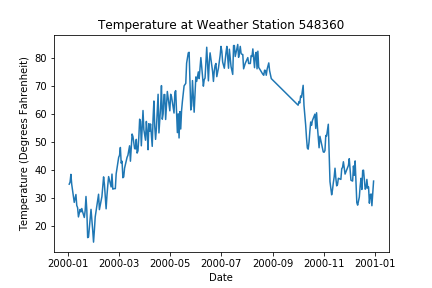
\includegraphics[scale=0.5]{temperature.png}

    The temperature at this weather station appears to peak in July at around 80 degrees Fahrenheit and drop to less than 20 degrees Fahrenheit in February. This suggests that this weather station is most likely located in the northern hemisphere.\footnote{\href{https://en.wikipedia.org/wiki/Northern_Hemisphere}{https://en.wikipedia.org/wiki/Northern\_Hemisphere}} \\

    \begin{itemize}
      \item Training and validation graphs based on the cost/loss function and evaluation metric (accuracy, F1, recall, RMSE, ...)
    \end{itemize}
  \end{itemize}
  \item Provide a timeline of the project to date and what the future work will entail. \\

  We hope to have data for the entire period from 1975 to 2019 by Friday, April 29th. We will then focus on developing separate models for each geographic region of the United States. We hope to be finished with the modeling portion of the project no later than Friday, May 6th so that we can spend the final week analyzing the results and editing the video presentation. \\

  \begin{itemize}
    \item Summarize completed and future work by using a \href{https://en.wikipedia.org/wiki/Gantt_chart}{\underline{Gantt chart}} to break down the tasks and due dates.
    \begin{itemize}
      \item Break down each task by specifying \textbf{who} is \textbf{doing what} and \textbf{when} it will be done.
      \item Avoid saying ``Everyone in the group'' is working on a single task. \\

      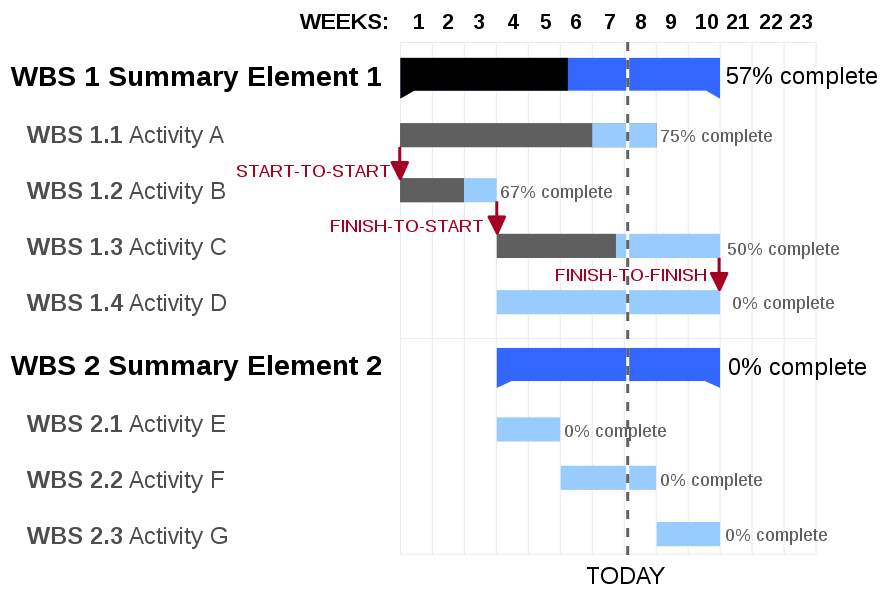
\includegraphics[scale=0.2]{gantt.png} \\

    \end{itemize}
  \end{itemize}
  \item Code
  \begin{itemize}
    \item Please provide code in a ZIP file or link to a GitHub repository. \textbf{Do \underline{not} submit your data set!}
    \item \textbf{If you have a private GitHub repository, please add @coatless.} \\

    https://github.com/emilyhasson/gsod-analysis \\

  \end{itemize}
\end{itemize}

\section{Contributions}

At the end of the progress report, please include a brief 1 - 2 sentence write-up of what each group member contributed to this stage of the project. Award each member with a percentage between 0 - 100 such that the sum of all percentages across group members will be equal to 100. \textbf{This section does not count toward the page limit.} \\

Lucas helped find and read in the data, even going so far as to write an automated Python script that pulls the data from the NOAA servers and then uploading it to Google Drive, our makeshift cloud storage solution. Lucas also created the initial \LaTeX\space file for the report. \\

Sam made several contributions to the report, including the preliminary results section. He also began the initial modeling phase of the project by fitting a logistic regression model to the 1975 data. \\

Emily wrote the introduction section of the report. She also helped find the dataset and created a shared GitHub repository, which you can access at the following URL: https://github.com/emilyhasson/gsod-analysis \\

Sam: 33.3\%

Lucas: 33.6\%

Emily: 33.1\%

\section{Grading}

The project will be graded according to a rubric. There will be no possibility for resubmission. To avoid grading surprises, please speak with a member of course staff about your draft during Office Hours prior to turning it in.

\section{References}

\href{https://en.wikipedia.org/wiki/Northern_Hemisphere}{https://en.wikipedia.org/wiki/Northern\_Hemisphere}

\section{Appendix}

\begin{table}[h!]
\centering
 \begin{tabular}{||c c c c c c||}
 \hline
  Station& Datetime &Temperature & \dots & Precip Flag \\ [0.5ex]
 \hline\hline
 548360 & 19750101 & 35.7 & \dots & G \\
 548360 & 19750101 & 35.7 & \dots & G \\
 548360 & 19750101 & 35.7 & \dots & G \\
 548360 & 19750101 & 35.7 & \dots & G \\
 \dots & \dots & \dots & \dots & \dots \\
 548360 & 19750101 & 35.7 & \dots & G \\
 548360 & 19750101 & 35.7 & \dots & G \\
 548360 & 19750101 & 35.7 & \dots & G \\
 548360 & 19750101 & 35.7 & \dots & G \\
 548360 & 19750101 & 35.7 & \dots & G \\[1ex]

 \hline
 \end{tabular}
 \caption{Sample of final dataset}
\end{table}

\end{document}
